\documentclass[10pt,a4paper]{article}

\usepackage[utf8]{inputenc}
\usepackage[T1]{fontenc}
\usepackage[brazil]{babel}
\usepackage{helvet}
\renewcommand{\familydefault}{\sfdefault}
\usepackage[top=16mm,bottom=18mm,left=15mm,right=15mm]{geometry}
\usepackage{xcolor}
\usepackage{graphicx}
\usepackage{booktabs}
\usepackage{tabularx}
\usepackage{array}
\usepackage{colortbl}
\usepackage{multicol}
\usepackage{lettrine}
\usepackage{fancyhdr}
\usepackage{lastpage}
\usepackage{hyperref}
\usepackage{parskip}

% ==============================================================================
% PALETA HARMONICA DINAMICA (INJETADA PELO R CONFORME CARTA OU DOSSIE)
% Mantem o Dourado Institucional (#C8942B) como DNA do Jornal Economico do TO
% ==============================================================================
\definecolor{corprimaria}{HTML}{4A1525}
\definecolor{corsecundaria}{HTML}{8C2D46}
\definecolor{douradoto}{HTML}{C8942B}
\definecolor{corfundo}{HTML}{F8F4F2}
\definecolor{cinzatexto}{HTML}{262D33}
\definecolor{cinzasuave}{HTML}{5A6570}
\definecolor{borda}{HTML}{D5DCE2}

\hypersetup{
    colorlinks=true,
    linkcolor=corprimaria,
    urlcolor=douradoto,
    pdftitle={Balanço Consolidado do Comércio Exterior Tocantinense: Superávit estrutural e avanço das cadeias agroindustriais},
    pdfauthor={Lorenzo Costa e Equipe | Jornal Econômico do Tocantins}
}

\setlength{\parindent}{0pt}
\setlength{\parskip}{5pt}
\renewcommand{\arraystretch}{1.24}

% Configuracao do formato de Periodico / Revista (2 Colunas)
\setlength{\columnsep}{18pt}
\setlength{\columnseprule}{0.4pt}
\renewcommand{\columnseprulecolor}{\color{borda}}

% Cabecalho e Rodape de Periodico
\pagestyle{fancy}
\fancyhf{}
\renewcommand{\headrulewidth}{0pt}
\renewcommand{\footrulewidth}{0.8pt}
\renewcommand{\footrule}{\hbox to\headwidth{\color{douradoto}\leaders\hrule height \footrulewidth\hfill}}

\fancyfoot[L]{\footnotesize\textcolor{corprimaria}{\textbf{JORNAL ECONÔMICO DO TOCANTINS}} \textcolor{cinzasuave}{$\vert$ DOSSIÊ ANUAL DE FECHAMENTO $\bullet$ Consolidado 2026}}
\fancyfoot[R]{\footnotesize\textcolor{cinzasuave}{Edição Periódica $\bullet$ Página \thepage\ de \pageref{LastPage}}}

% Comando para Titulos de Secao dentro das Colunas da Revista
\newcommand{\secaoperiodico}[1]{%
  \vspace{4pt}%
  \noindent\colorbox{corfundo}{%
    \parbox{\dimexpr\columnwidth-2\fboxsep\relax}{%
      \vspace{3pt}%
      \textcolor{douradoto}{\rule{4pt}{9pt}}\hspace{6pt}%
      \textcolor{corprimaria}{\textbf{\small \MakeUppercase{#1}}}%
      \vspace{2pt}%
    }%
  }\\[-2pt]%
  \noindent{\color{corprimaria}\rule{\columnwidth}{1pt}}%
  \vspace{3pt}\par%
}

\begin{document}
\color{cinzatexto}

% ==============================================================================
% MASTHEAD DE REVISTA / PERIODICO ECONOMICO
% ==============================================================================
\noindent{\scriptsize\textcolor{corprimaria}{\textbf{PUBLICAÇÃO PERIÓDICA DE ANÁLISE CONJUNTURAL E ESTRUTURAL}} \hfill \textcolor{cinzasuave}{\textbf{ANUÁRIO SETORIAL • COMÉRCIO EXTERIOR $\bullet$ 29/10/2026}}}\\[-4pt]
\noindent{\color{douradoto}\rule{\textwidth}{1.2pt}}\\[-1pt]
\noindent\colorbox{corprimaria}{%
  \parbox{\dimexpr\textwidth-2\fboxsep\relax}{%
    \vspace{7pt}%
    \begin{tabularx}{\linewidth}{@{}X r@{}}
      {\fontsize{16}{19}\selectfont\textbf{\textcolor{white}{JORNAL ECONÔMICO DO TOCANTINS}}} &
      \colorbox{douradoto}{\textbf{\footnotesize\textcolor{corprimaria}{\hspace{6pt}DOSSIÊ ANUAL • COMÉRCIO EXTERIOR\hspace{6pt}}}} \\[5pt]
      {\footnotesize\textcolor{douradoto}{\textbf{Série Periódica de Estudos Econômicos $\bullet$ Balanço Consolidado dos Resultados Mensais e Trimestrais do Tocantins}}} &
      {\footnotesize\textcolor{white}{Referência: \textbf{Consolidado 2026}}}
    \end{tabularx}%
    \vspace{5pt}%
  }%
}\\[-2pt]
\noindent{\color{douradoto}\rule{\textwidth}{2.6pt}}

\vspace{6pt}

% ==============================================================================
% MANCHETE DE CAPA, LINHA-FINA E CREDITO EDITORIAL
% ==============================================================================
{\fontsize{16}{20}\selectfont\textbf{\textcolor{corprimaria}{Balanço Consolidado do Comércio Exterior Tocantinense: Superávit estrutural e avanço das cadeias agroindustriais}}}\\[4pt]
{\normalsize\textcolor{cinzasuave}{\textit{Análise integrada da pauta exportadora, dependências de insumos importados e posicionamento competitivo do Estado no mercado internacional}}}\\[5pt]
\noindent{\color{borda}\rule{\textwidth}{0.5pt}}\\[-1pt]
{\footnotesize\textcolor{corprimaria}{\textbf{Corpo Editorial:}} \textcolor{cinzatexto}{Lorenzo Costa e Equipe | Jornal Econômico do Tocantins} \hfill \textcolor{corprimaria}{\textbf{Fontes Oficiais:}} \textcolor{cinzatexto}{Comex Stat / MDIC}}\\[-3pt]
\noindent{\color{borda}\rule{\textwidth}{0.5pt}}

\vspace{3pt}

% Lead / Sintese Executiva em Estilo de Revista
\noindent\fcolorbox{corprimaria}{corfundo}{%
  \parbox{\dimexpr\textwidth-2\fboxsep-2\fboxrule\relax}{%
    \vspace{3pt}%
    \textcolor{douradoto}{\rule{6pt}{6pt}}\hspace{5pt}\textbf{\textcolor{corprimaria}{SÍNTESE EXECUTIVA DA EDIÇÃO:}} O Tocantins consolida saldo comercial superavitário de US\$ 2,06 bilhões na parcial consolidada, sustentado pela força da soja em grãos, da proteína bovina refrigerada/congelada e do milho, enquanto a pauta importadora confirma forte investimento em fertilizantes e maquinário produtivo.%
    \vspace{3pt}%
  }%
}

\vspace{4pt}

% ==============================================================================
% FAIXA DE INDICADORES-CHAVE (KPIs NA PALETA DO PERIODICO)
% ==============================================================================
\noindent\colorbox{corprimaria}{\parbox[t][1.32cm][c]{0.225\textwidth}{\centering\scriptsize\textcolor{white}{\textbf{Exportações (FOB)}}\\[3pt]{\large\textbf{\textcolor{douradoto}{US\$ 200,89 Mi}}}}}\hfill\colorbox{corprimaria}{\parbox[t][1.32cm][c]{0.225\textwidth}{\centering\scriptsize\textcolor{white}{\textbf{Importações (FOB)}}\\[3pt]{\large\textbf{\textcolor{douradoto}{US\$ 63,95 Mi}}}}}\hfill\colorbox{corprimaria}{\parbox[t][1.32cm][c]{0.225\textwidth}{\centering\scriptsize\textcolor{white}{\textbf{Saldo Comercial}}\\[3pt]{\large\textbf{\textcolor{douradoto}{+ US\$ 136,94 Mi}}}}}\hfill\colorbox{corprimaria}{\parbox[t][1.32cm][c]{0.225\textwidth}{\centering\scriptsize\textcolor{white}{\textbf{Corrente Total}}\\[3pt]{\large\textbf{\textcolor{douradoto}{US\$ 264,84 Mi}}}}}
\vspace{5pt}


% ==============================================================================
% CORPO EDITORIAL EM 2 COLUNAS (FORMATO DE REVISTA / PERIODICO ECONOMICO)
% ==============================================================================
\begin{multicols}{2}
\secaoperiodico{1. Panorama Estatístico do Período}

No período de referência (Consolidado 2026), a corrente total de comércio exterior do Estado do Tocantins (soma das exportações e importações) atingiu US\$ 264,84 milhões. As vendas externas somaram US\$ 200,89 milhões (US\$ 200,89 Mi), ao passo que as aquisições de produtos estrangeiros totalizaram US\$ 63,95 milhões (US\$ 63,95 Mi). Como resultado, a balança comercial tocantinense apresentou expressivo superávit comercial e acumulou geração líquida positiva de divisas da ordem de US\$ 136,94 milhões (+ US\$ 136,94 Mi), com índice de cobertura de 3,1x (exportações equivalentes a 3,1 vezes o valor importado).

\vspace{4pt}

Na decomposição setorial da pauta exportadora por posição SH4, o desempenho foi puxado por Carnes de animais da espécie bovina, congeladas, que movimentou US\$ 50,28 milhões (42,2\% do top 3 exportador), seguido por Soja, mesmo triturada com US\$ 36,35 milhões (30,5\%). Pela ótica das importações, a demanda estadual concentrou-se em Adubos (fertilizantes) azotados (US\$ 34,82 milhões, ou 76,9\% dos principais itens), refletindo a estrutura de custos de insumos produtivos. Geograficamente, China consolidou-se como o principal destino individual das exportações estaduais (US\$ 46,97 milhões, respondendo por 23,4\% do total exportado), enquanto China liderou a origem das compras externas (US\$ 15,98 milhões).

\secaoperiodico{2. Análise de Conjuntura da Equipe}

\lettrine[lines=2, lhang=0.05, nindent=2pt]{\textcolor{corprimaria}{\textbf{M}}}{\textbf{AIS}} do que observar as oscilações mensais típicas da sazonalidade agrícola, a leitura do consolidado anual do comércio exterior tocantinense revela a maturidade produtiva alcançada pelo Estado dentro da fronteira agrícola do MATOPIBA. A geração de um saldo positivo robusto funciona como um colchão de liquidez em moeda forte que irriga toda a cadeia de serviços logísticos, transporte rodoviário/ferroviário, armazenagem e comércio nos municípios polos.

\vspace{4pt}

Um segundo ponto que merece atenção da nossa equipe é a qualidade do fluxo de importações. Diferentemente de estados cuja pauta importadora é dominada por bens de consumo final, o Tocantins importa majoritariamente bens intermediários essenciais e bens de capital — notadamente adubos, fertilizantes e máquinas agrícolas. Em termos econômicos, isso significa que a saída de divisas pela via das importações não representa vazamento improdutivo de renda, mas sim formação bruta de capital e preparação tecnológica para a safra seguinte.

\vspace{4pt}

Por outro lado, a elevada concentração das vendas externas em poucos mercados asiáticos — com destaque absoluto para a China — mantém o Estado exposto a choques de demanda externa e oscilações nos prêmios portuários. Ainda assim, a presença consolidada da carne bovina e do milho na pauta demonstra um avanço gradual na agregação de valor frente à monocultura exportadora observada há uma década.

\secaoperiodico{3. Perspectivas e Cenários}

Para os próximos trimestres, a manutenção de um câmbio competitivo em patamares favoráveis ao exportador tende a compensar eventuais acomodações nas cotações internacionais das commodities em dólar na Bolsa de Chicago (CBOT).

\vspace{4pt}

O principal vetor estrutural a ser monitorado pelos agentes econômicos locais é a redução do custo logístico no corredor Centro-Norte (Ferrovia Norte-Sul e saída pelos portos do Arco Norte, como Itaqui/MA), fator decisivo para ampliar a margem líquida do produtor tocantinense e atrair novas plantas de processamento agroindustrial para o território estadual.
\end{multicols}

\vspace{4pt}

% ==============================================================================
% PAINEL DE EVIDENCIA EMPIRICA (GRAFICOS E TABELAS EM LARGURA TOTAL)
% ==============================================================================
\noindent\fcolorbox{borda}{white}{%
  \parbox{\dimexpr\textwidth-2\fboxsep-2\fboxrule\relax}{%
    \vspace{3pt}%
    \noindent\colorbox{corprimaria}{%
      \parbox{\dimexpr\linewidth-2\fboxsep\relax}{%
        \vspace{3pt}\hspace{4pt}\textcolor{douradoto}{\rule{6pt}{6pt}}\hspace{6pt}%
        \textbf{\footnotesize\textcolor{white}{PAINEL DE EVIDÊNCIA EMPÍRICA $\bullet$ GRÁFICOS E TABELAS CONSOLIDADAS DA EDIÇÃO}}\vspace{3pt}%
      }%
    }\\[6pt]
    \begin{center}
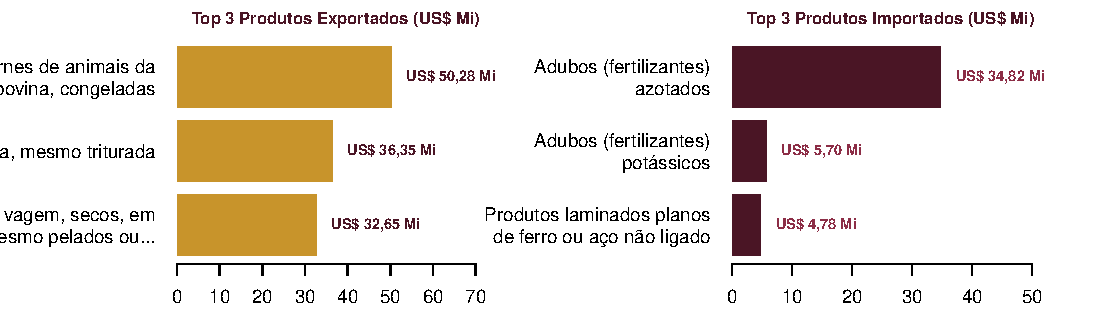
\includegraphics[width=0.98\linewidth]{boletins/build/fig_2026_10_fechamento_comex.pdf}
\end{center}
\vspace{1pt}
\noindent\begin{minipage}{\linewidth}
{\footnotesize
\noindent\textbf{\textcolor{corprimaria}{Tabela 1 — Principais Parceiros Comerciais do Tocantins (Destinos de Exportação e Origens de Importação)}}\\[2pt]
\begin{tabularx}{\linewidth}{@{}X r r @{\hspace{16pt}} X r r@{}}
\toprule
\rowcolor{corprimaria} \textcolor{white}{\textbf{Destino (Exportação)}} & \textcolor{white}{\textbf{US\$ Mi}} & \textcolor{white}{\textbf{Part. (\%)}} & \textcolor{white}{\textbf{Origem (Importação)}} & \textcolor{white}{\textbf{US\$ Mi}} & \textcolor{white}{\textbf{Part. (\%)}} \\
\midrule
China & 46,97 & 23,4\% & China & 15,98 & 25,0\% \\
Índia & 33,59 & 16,7\% & Nigéria & 14,93 & 23,3\% \\
Canadá & 16,57 & 8,2\% & Venezuela & 14,67 & 22,9\% \\
Egito & 16,18 & 8,1\% & Canadá & 5,71 & 8,9\% \\
Espanha & 10,32 & 5,1\% & Estados Unidos & 4,48 & 7,0\% \\
Suíça & 8,20 & 4,1\% & Vietnã & 3,90 & 6,1\% \\
\bottomrule
\end{tabularx}
}
\end{minipage}
\vspace{2pt}

  }%
}

\vfill
\noindent{\color{douradoto}\rule{\textwidth}{1pt}}\\[-2pt]
{\scriptsize\textcolor{cinzasuave}{\textbf{Expediente e Nota Metodológica:} Ministério do Desenvolvimento, Indústria, Comércio e Serviços (Comex Stat / MDIC). Elaboração: Jornal Econômico do Tocantins. Publicação diagramada em formato de periódico (2 colunas) pelo Sistema Editorial Híbrido (R + LaTeX) do Jornal Econômico do Tocantins.}}

\end{document}
